\documentclass{rapportIMT}
\usepackage[T1]{fontenc}
\usepackage[utf8]{inputenc}
\usepackage[english]{babel}
\usepackage{lipsum}
\usepackage{awesomebox}
\usepackage{tcolorbox}
\usepackage{longtable}
\usepackage{multirow}
\usepackage{tabularx}
\usepackage{booktabs}
\usepackage{tikz}
\usepackage{pgfplots}
\pgfplotsset{compat=1.18}
\usepackage{pdflscape}
\usepackage{adjustbox}
\usepackage{pdfpages}
\renewcommand{\arraystretch}{1.25}
\usepackage[dvipsnames]{xcolor}
\usepackage{colortbl}
\usepackage{array}
\usepackage{changepage}
\usepackage{caption}
\usepackage{subcaption}
\usepackage{graphicx}
\usepackage{svg}
\usepackage{enumitem}
\usepackage{amsmath}
\usetikzlibrary{shapes.geometric, arrows.meta, positioning, calc, decorations.pathreplacing, babel, fit, backgrounds}

% Dossier des figures
\graphicspath{{./}{figures/}{logos/}{../../figures/}{../../logos/}}

% Couleurs du template
\definecolor{doctoblue}{RGB}{20,79,158}
\definecolor{doctolight}{RGB}{210,228,247}
\definecolor{alertred}{RGB}{176,42,42}
\definecolor{alertlight}{RGB}{248,222,222}
\definecolor{okgreen}{RGB}{38,120,72}
\definecolor{oklight}{RGB}{222,240,228}
\definecolor{greyline}{RGB}{120,120,120}

% Styles TikZ communs
\tikzset{
  bx/.style={rectangle, rounded corners, draw=doctoblue, fill=doctolight, text width=3cm, align=center, minimum height=1.2cm, font=\small},
  bxd/.style={rectangle, rounded corners, draw=doctoblue, fill=doctoblue, text=white, text width=3cm, align=center, minimum height=1.2cm, font=\small},
  bxr/.style={rectangle, rounded corners, draw=alertred, fill=alertlight, text width=3cm, align=center, minimum height=1.2cm, font=\small},
  bxg/.style={rectangle, rounded corners, draw=okgreen, fill=oklight, text width=3cm, align=center, minimum height=1.2cm, font=\small},
  ar/.style={-{Latex[length=3mm]}, thick, doctoblue},
  arr/.style={-{Latex[length=3mm]}, thick, alertred},
  arg/.style={-{Latex[length=3mm]}, thick, okgreen}
}

% Encadré de synthèse (même style que le template)
\newtcolorbox{synthese}{colback=doctolight!35, colframe=doctoblue, boxrule=0.5pt, arc=2pt,
  left=6pt, right=6pt, top=4pt, bottom=4pt, fonttitle=\bfseries\small,
  title={Key strategic recommendations}}

% Encadré « Answer to the board »
\newtcolorbox{reponse}{colback=doctolight!35, colframe=doctoblue, boxrule=0.5pt, arc=2pt,
  left=6pt, right=6pt, top=4pt, bottom=4pt, fonttitle=\bfseries\small,
  title={Answer to the board}}

% --- Marges standard 2,5 cm ---
\geometry{a4paper, margin=2.5cm}

% --- Police Times New Roman ---
\usepackage{newtxtext,newtxmath}

% --- Interligne 1,12 ---
\usepackage{setspace}
\setstretch{1.12}

% Figures plus compactes
\setlength{\textfloatsep}{8pt plus 2pt minus 2pt}
\setlength{\intextsep}{6pt plus 2pt minus 2pt}
\captionsetup{font=small, labelfont=bf, skip=3pt}

% Macros utilitaires
\newcommand{\eur}{\texteuro{}}
\newcommand{\Meur}{\,M\eur}
\newcommand{\pc}{\,\%}

% Liens
\hypersetup{
  colorlinks=true,
  linkcolor=black,
  citecolor=doctoblue,
  urlcolor=doctoblue
}

\begin{document}
\newcolumntype{M}[1]{>{\raggedright}m{#1}}
\newcolumntype{C}[1]{>{\centering}m{#1}}

%----------- Informations du rapport ---------

\titre{Tasko: what really drives growth before the Series A?}
\trigrammemention{2026 - 2027}
\master{\Large Data \& Digital Society}

\eleve{
    \textbf{Groupe 15} \\
    Joe \textsc{El-Hajj} \\
    Colomban \textsc{Boisseau} \\
    Mouad \textsc{Chouki} \\
    Maxime \textsc{Philippon}
}

\dates{2026 - 2027}

%----------- Initialisation -------------------

\fairemarges
\fairepagedegarde

\newpage

\renewcommand{\contentsname}{Contents}
{\small\setstretch{1.0}\tableofcontents}
\vspace{0.4cm}

\newpage

\small

% ==================================================================
\begin{reponse}
\small
Tasko's founders are right to believe in product-led growth, but the product does its work after the sign-up, not before it. A workspace that gathers a team of three is 2.5 times more likely to pay, and the existing base already feeds a guest loop that brings in one new workspace out of five. Paid search, the largest marketing line, tells the opposite story: it buys sign-ups at a steady 55\eur{} each, but few of them become teams, so its LTV\,:\,CAC barely reaches 1.16 on revenue and its payback stretches to 31.5 months. The single most important event of the period was the onboarding change of September 2025, which lifted activation by 20 points and conversion by 2.7 points. Looking ahead, our model places June 2027 MRR between 42 and 109\,k\eur{}, and the gap between these outcomes is driven by conversion and team size far more than by advertising budget.
\end{reponse}

% ==================================================================
\section{Data and method}
\label{sec:data}

We work on eighteen months of activity, from January 2025 to June 2026, as extracted from production on 30 June 2026. The four files arrived uncleaned, so each correction was written as an explicit rule and counted. The full log is given in Appendix~\ref{sec:app-log} (Table~\ref{tab:log}). Three definitions underpin everything that follows:
\begin{itemize}[nosep,topsep=2pt]
  \item \textbf{Activation}: at least two teammates join the workspace within 30 days of its creation, which, together with the owner, makes a team of three. Section~\ref{sec:funnel} explains why we chose this threshold.
  \item \textbf{Conversion}: an upgrade to a paid plan (Pro at 8\eur{} or Business at 12\eur{} per seat and per month) within 90 days. Since no workspace took longer than 89 days to upgrade, only cohorts created before April 2026 can be fully observed. We call them mature cohorts ($N = 7{,}556$).
  \item \textbf{Churn}: a paying workspace whose last invoice is earlier than June 2026. Billing histories contain no gaps, so this reading is unambiguous.
\end{itemize}
Finally, the data pack gives no gross margin. All lifetime values are therefore revenue LTVs ($\text{LTV} = \text{ARPA}/\text{churn}$), and should be read as upper bounds.

% ==================================================================
\section{Funnel and growth loop}
\label{sec:funnel}

\textbf{Activation is the hinge of the funnel.} Workspaces with no teammate, or only one, convert at a modest 5.3--5.9\pc{}. As soon as a second teammate joins, conversion more than doubles to 12.5\pc{}, and it keeps climbing to 17.7\pc{} for teams of six or more (Figure~\ref{fig:funnel}, right). The jump is sharp enough to serve as Tasko's Aha moment in the AARRR sense: the point at which a user stops trying the product alone and starts using it with a team.

\begin{figure}[htbp]
  \centering
  \begin{subfigure}{0.52\textwidth}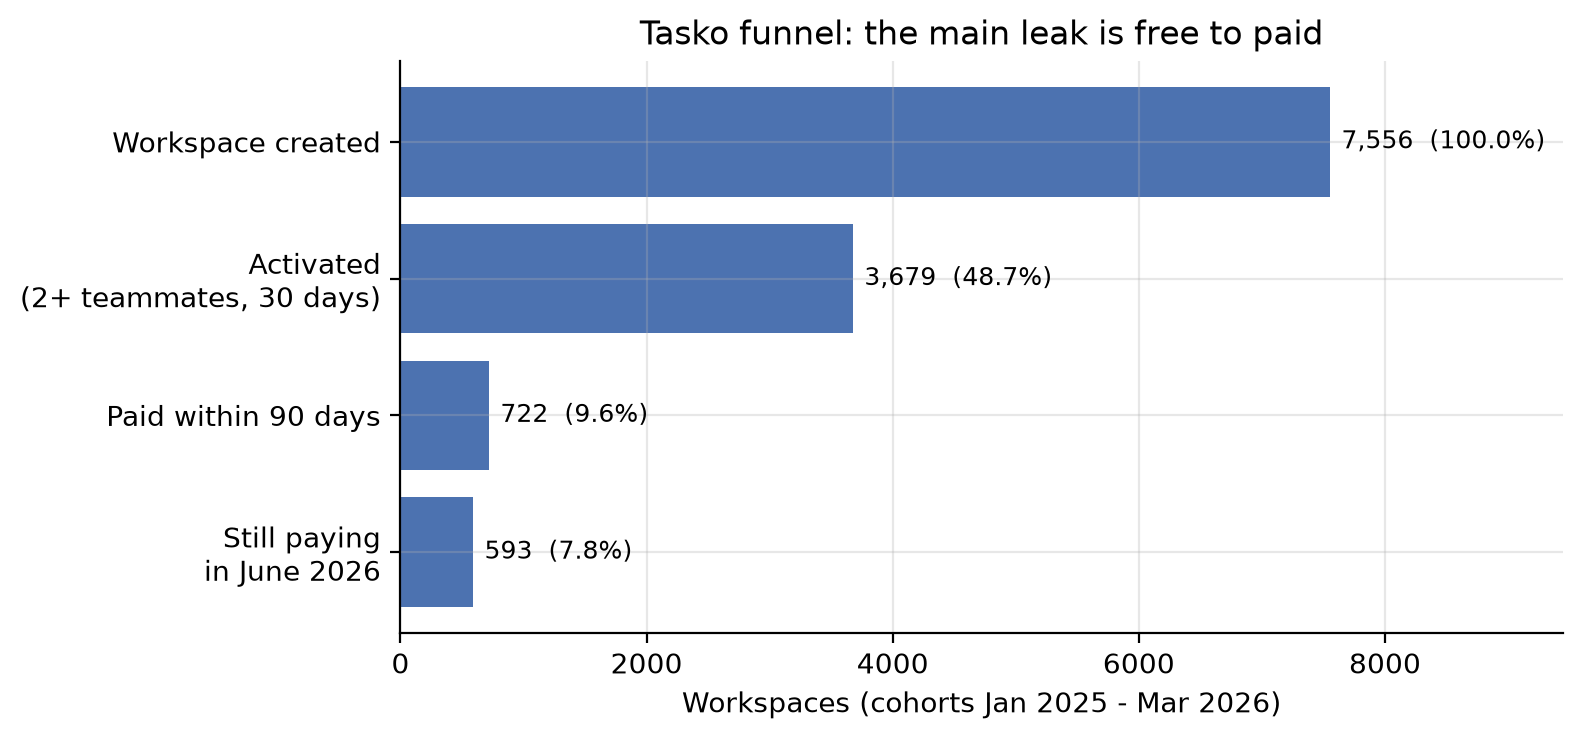
\includegraphics[width=\linewidth]{fig02_funnel.png}\end{subfigure}\hfill
  \begin{subfigure}{0.45\textwidth}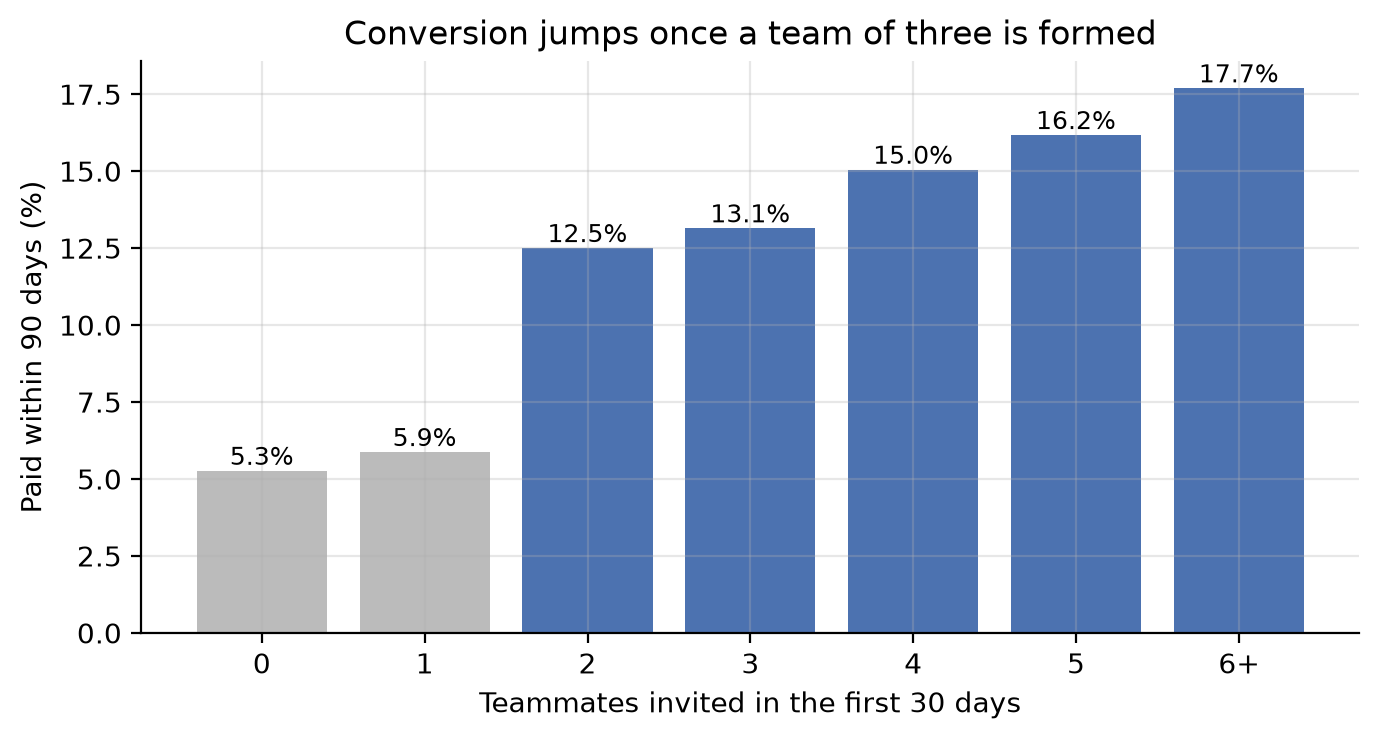
\includegraphics[width=\linewidth]{fig01_aha_moment.png}\end{subfigure}
  \caption{Funnel of mature cohorts Jan 2025 -- Mar 2026 (left) and 90-day conversion by teammates invited in the first 30 days (right).}
  \label{fig:funnel}
\end{figure}

Following the 7,556 mature workspaces down the funnel, 48.7\pc{} become activated, 9.6\pc{} pay within 90 days, and 7.8\pc{} are still paying in June 2026. The last step is reassuring: 82\pc{} of the workspaces that start paying keep doing so. \textbf{The value is therefore lost between free and paid}, and activation largely decides what happens at that step. Activated workspaces convert at 13.8\pc{} against 5.6\pc{} for the others, and they account for 70\pc{} of all conversions.

\textbf{A real loop, still modest, but compounding.} Some guests invited into a workspace later open one of their own, which the data records as \texttt{invite\_loop}. This channel grew from nothing in January 2025 to \textbf{19.8\pc{} of new workspaces in June 2026}, while the share of paid search fell from 32.4\pc{} to 25.8\pc{}. Outbound invitations are not logged, so we cannot compute $K = i \times c$ as in the course. Instead, we measure the effective virality directly. Each workspace generated \textbf{0.086 new workspaces within 180 days before mid-September 2025, and 0.123 afterwards}. With $K$ well below 1, the loop cannot replace acquisition, but it does amplify it. It is also slow, with a median delay of 146 days between a workspace and the one it gives rise to. More surprisingly, its rate (about 0.10) is the same whatever the activation, payment status or channel of the origin workspace. What feeds the loop is simply the size of the base, which grows by 1.5--2.2\pc{} each month through this channel alone, and this is precisely why its output compounds over time.

% ==================================================================
\section{Channels and segments}
\label{sec:channels}

On every early indicator, paid search trails the other channels. Only 29.2\pc{} of its workspaces become activated, against 49.6--59.2\pc{} elsewhere. Only 6.4\pc{} convert within 90 days, against 10.7--11.8\pc{} for organic, SEO and the loop. The teams it brings are also smaller, with 3.1 seats and an ARPA of 27.5\eur{} against 35.0--38.2\eur{}. Its only advantage, discussed in Section~\ref{sec:ue}, is that its paying customers churn less.

\begin{figure}[htbp]
  \centering
  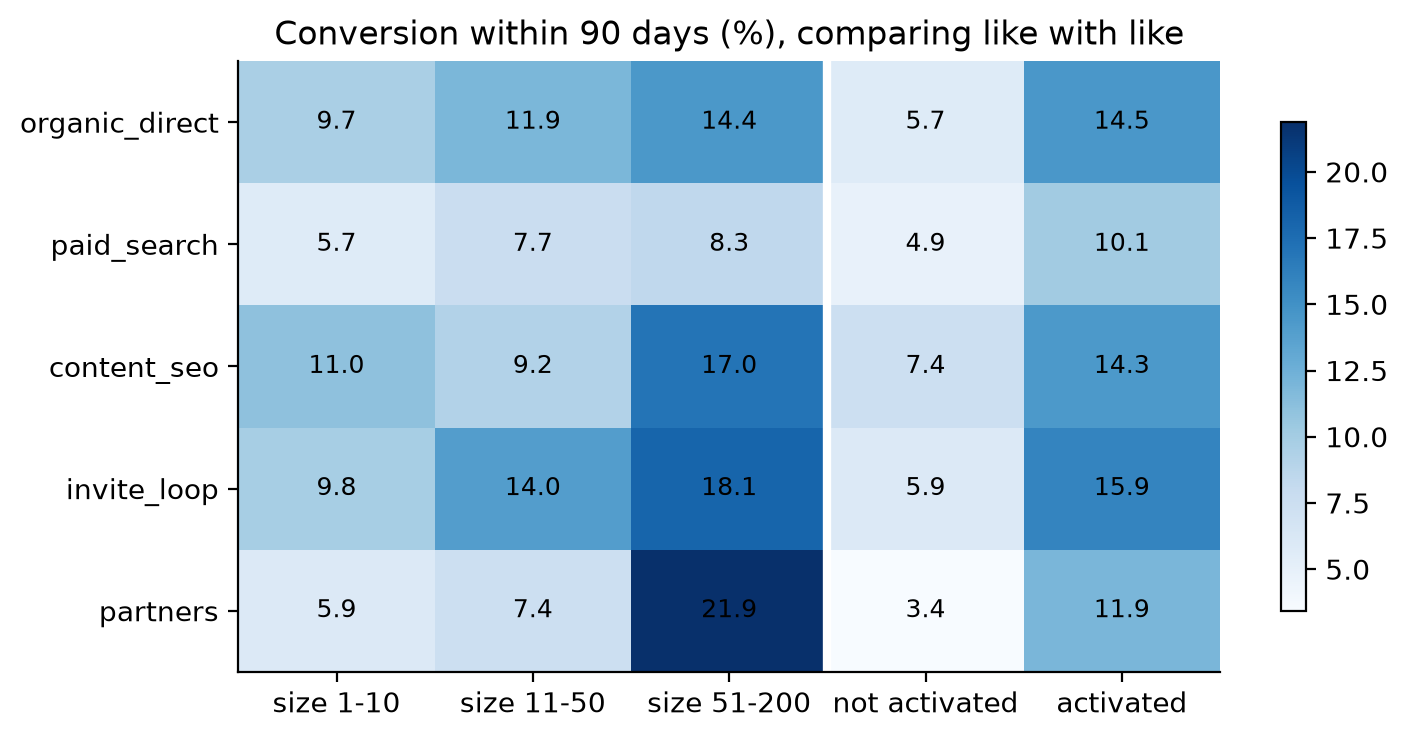
\includegraphics[width=0.62\textwidth]{fig06_like_for_like.png}
  \caption{Like-for-like 90-day conversion (\%) by channel, within company size and within activation status.}
  \label{fig:lfl}
\end{figure}

A natural objection is that paid search might simply attract a different kind of company. The data rules this out (Figure~\ref{fig:lfl}). \textbf{The gap survives a like-for-like comparison}: all channels bring almost the same mix of company sizes (about 60\,/\,29\,/\,9\pc{}), and paid search still converts least among companies of 1--10 employees (5.7\pc{}) and of 51--200 employees (8.3\pc{}). The difference persists even \textbf{among activated workspaces}, where paid search converts at 10.1\pc{} against 14.3--15.9\pc{} for organic, SEO and the loop. In other words, its users are less likely to form a team, and less likely to pay even when they do. The other channels, by contrast, look very much alike once compared on equal terms.

Across segments, \textbf{company size is the strongest driver of value}. A workspace of 51--200 employees holds 7.0 seats on average, brings in 66\eur{} a month and churns at only 1.2\pc{} per month. A team of 1--10, by contrast, holds 2.6 seats, brings 21\eur{} and churns at 4.4\pc{}. The plan points in the same direction, with Business accounts churning less than Pro ones (2.1\pc{} against 3.5\pc{}).

% ==================================================================
\section{Unit economics}
\label{sec:ue}

\begin{table}[htbp]
\centering
\footnotesize\renewcommand{\arraystretch}{1.15}
\adjustbox{max width=\linewidth}{%
\begin{tabular}{lrrrrrr}
\toprule
Channel & Cost per sign-up & CAC (paying) & ARPA & Monthly churn & Revenue LTV & LTV\,:\,CAC \;/\; Payback \\
\midrule
Paid search  & 55\eur & 864\eur   & 27.5\eur & 2.7\,\% & 1,007\eur & 1.16 \;/\; 31.5 months \\
Content SEO  & 40\eur & 357\eur   & 37.8\eur & 3.7\,\% & 1,022\eur & 2.86 \;/\; 9.5 months \\
Partners     & 93\eur & 1,210\eur & 38.2\eur & 4.6\,\% & 830\eur   & 0.69 \;/\; 31.7 months \\
\bottomrule
\end{tabular}}
\caption{Unit economics of the paid channels (cohorts Jan 2025 -- Mar 2026). Organic direct and invite loop carry no spend.}
\label{tab:ue}
\end{table}

\begin{figure}[htbp]
  \centering
  \begin{subfigure}{0.48\textwidth}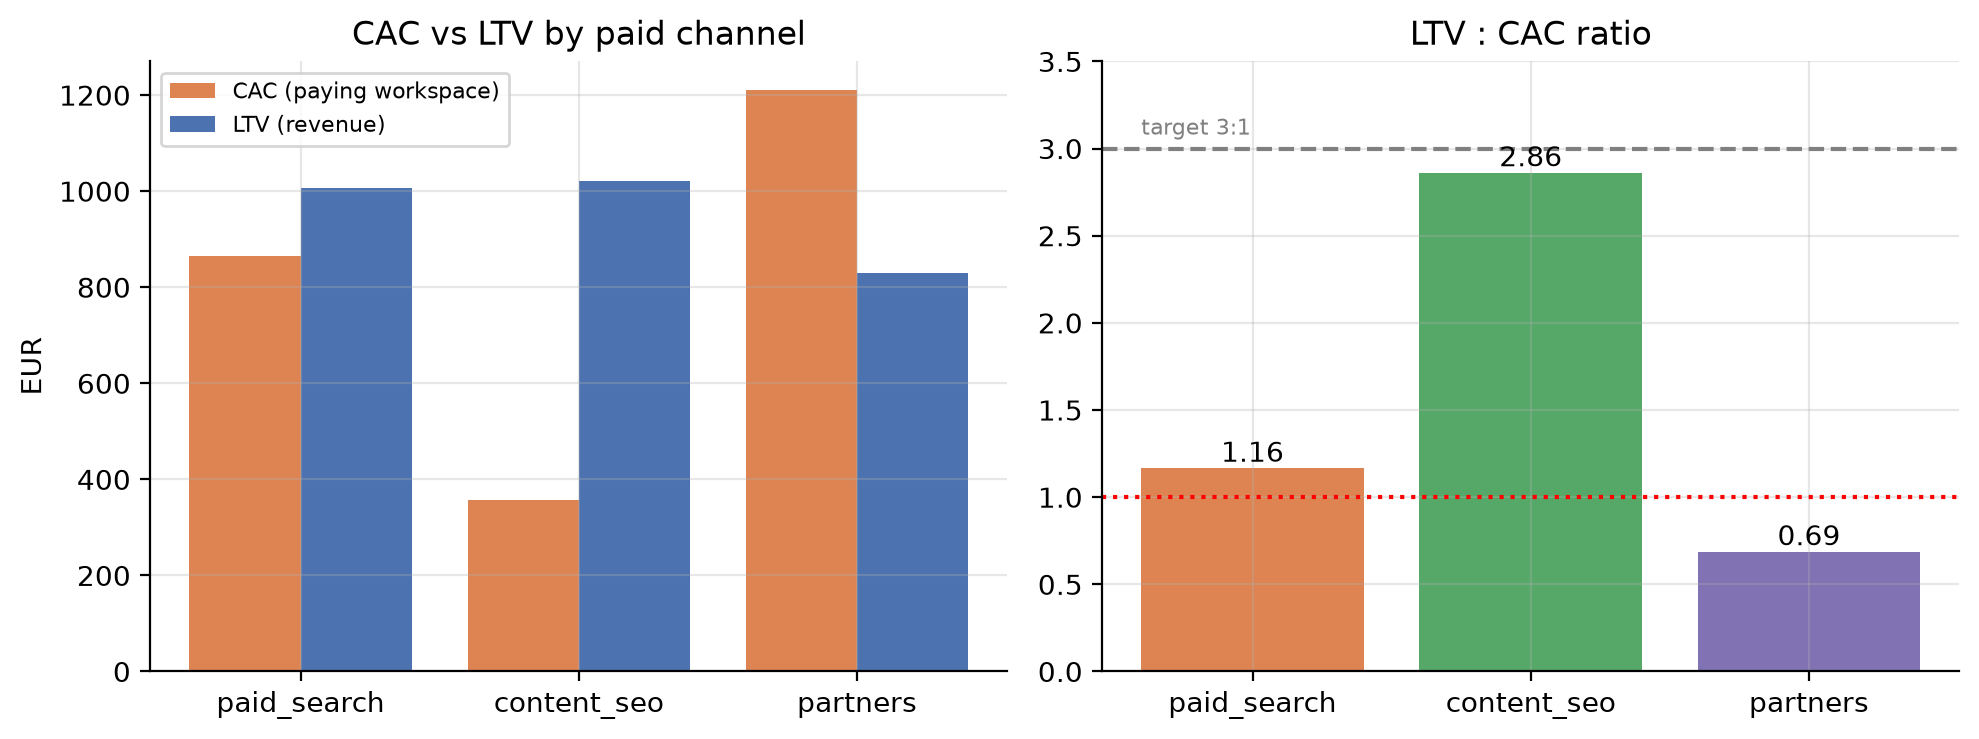
\includegraphics[width=\linewidth]{fig07_unit_economics.png}\end{subfigure}\hfill
  \begin{subfigure}{0.48\textwidth}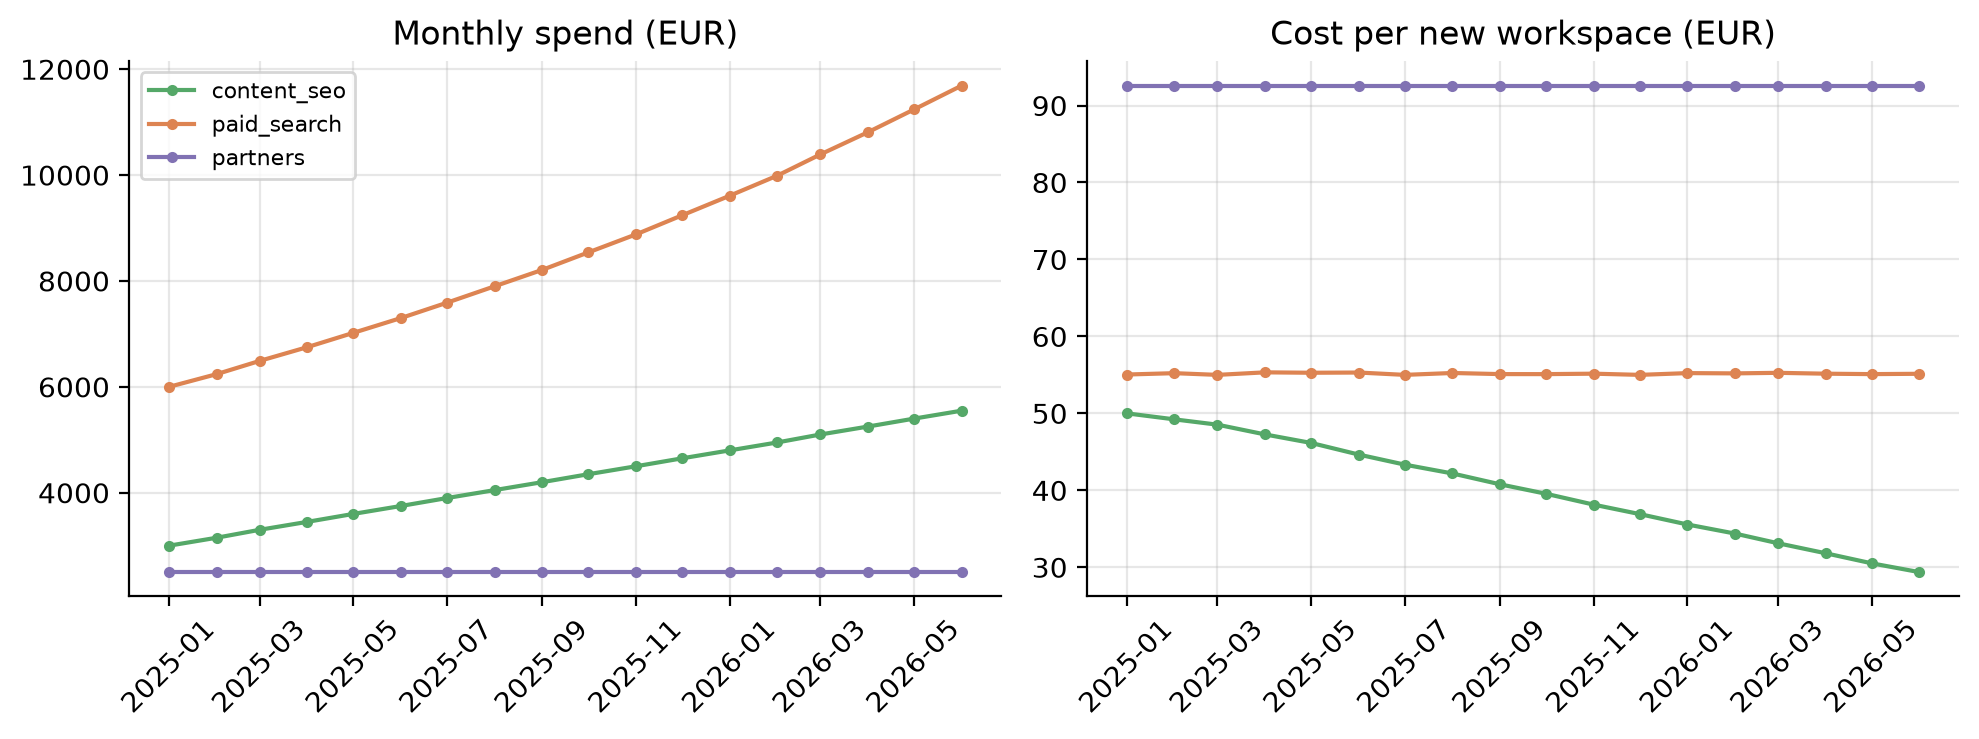
\includegraphics[width=\linewidth]{fig08_spend_and_cost_per_signup.png}\end{subfigure}
  \caption{CAC vs revenue LTV and LTV\,:\,CAC ratio (left), monthly spend and cost per new workspace over time (right).}
  \label{fig:ue}
\end{figure}

The three paid channels lead to very different conclusions (Table~\ref{tab:ue}). \textbf{Content SEO} comes close to the 3\,:\,1 benchmark of the course, with a ratio of 2.86 and a payback under ten months. It also improves with time: its cost per sign-up fell from 50\eur{} to 29\eur{} over the period, as published content kept attracting visitors (Figure~\ref{fig:ue}). \textbf{Paid search} is much more fragile. Its ratio of 1.16 is computed on revenue, so it falls below 1 as soon as the gross margin is under 86\pc{}, and its payback of 31.5 months is longer than most cohorts have been observed. What makes the case instructive is that paid search customers are not worse customers: they churn the least (2.7\pc{} a month), so their LTV of 1,007\eur{} is on a par with that of SEO (1,022\eur{}). The whole gap lies in the cost of acquiring them, 864\eur{} against 357\eur{}. Its budget almost doubled over the period ($\times 1.95$) while the cost per sign-up stayed at 55\eur{}: this channel grows strictly in proportion to what is spent on it. \textbf{Partners}, finally, destroy value, with a ratio of 0.69 for a flat 2,500\eur{} a month that brings in 27 sign-ups. Because half of the paying workspaces cost nothing to acquire (organic direct and the loop), the blended CAC is only 302\eur{}, against 642\eur{} for the paid channels alone.

\textbf{Retention, on the other hand, is sound.} Monthly churn is around 3\pc{}, between 76\pc{} and 94\pc{} of paying workspaces are still billed after six months, and recent cohorts hold up no worse than older ones. MRR reached \textbf{24,512\eur{} in June 2026}, from 654 paying workspaces. ARPA rose from 31.6\eur{} to 37.5\eur{} during the first half of 2026, but this does not come from existing customers growing: the six-month net revenue retention of the December 2025 base is 95\pc{}, as the 19\pc{} of accounts that added seats do not fully offset those that left. The increase therefore comes mostly from new accounts that start with larger teams.

% ==================================================================
\section{What changed, and what it caused}
\label{sec:change}

\begin{figure}[htbp]
  \centering
  \begin{subfigure}{0.47\textwidth}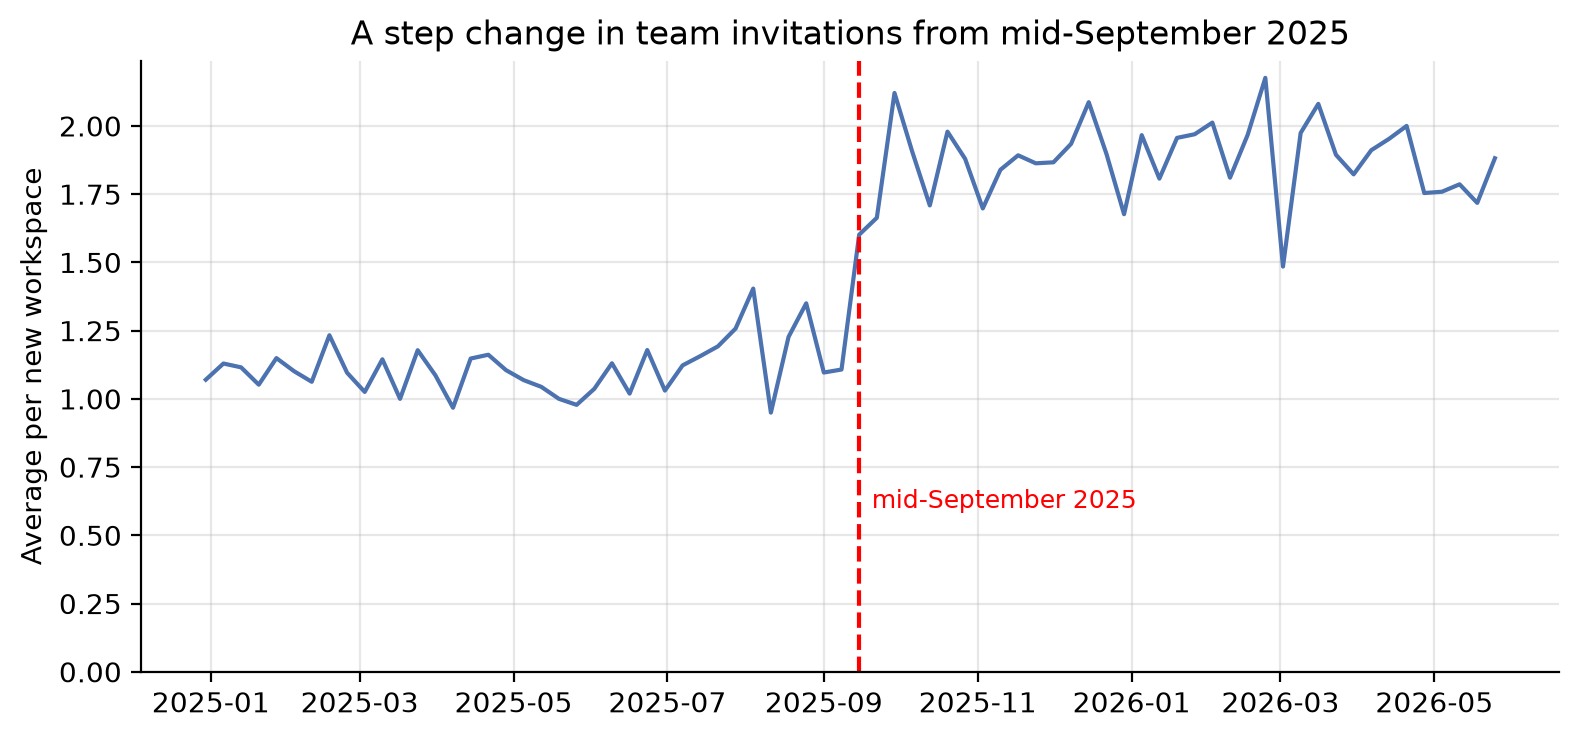
\includegraphics[width=\linewidth]{fig11_change_detection.png}\end{subfigure}\hfill
  \begin{subfigure}{0.50\textwidth}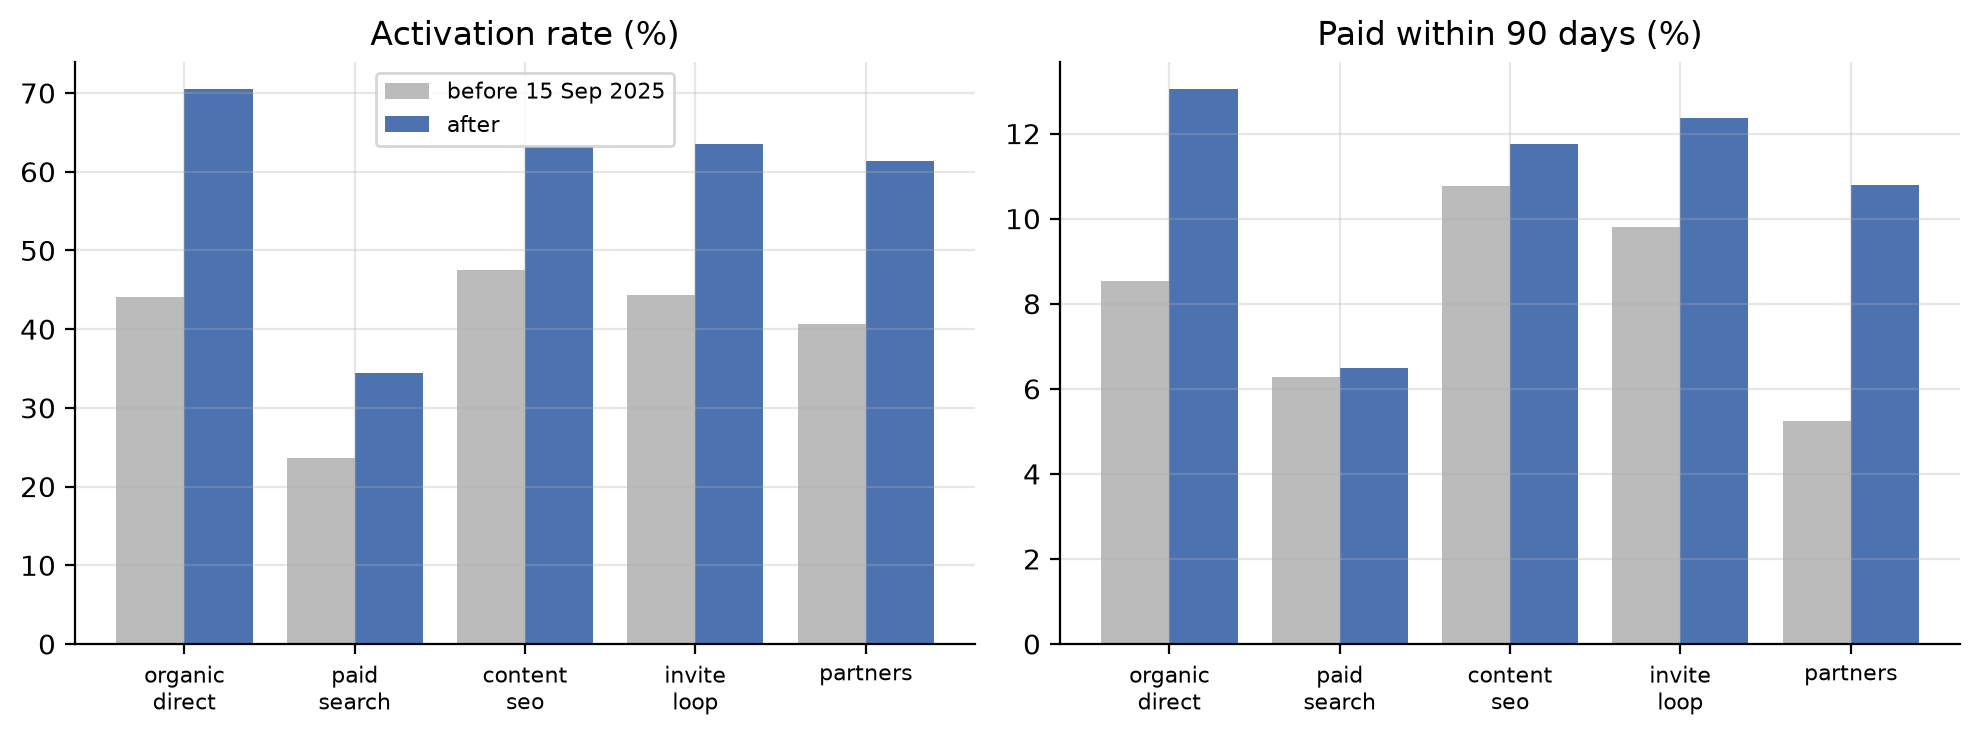
\includegraphics[width=\linewidth]{fig12_before_after.png}\end{subfigure}
  \caption{Teammates invited in the first week by creation week (left), activation and conversion before/after 15 Sep 2025 (right).}
  \label{fig:change}
\end{figure}

One date stands out over the eighteen months. In the second half of September 2025, the number of teammates invited during a workspace's first week jumps from about 1.1 to about 1.9, and never falls back (Figure~\ref{fig:change}). The data does not say what happened, but a lasting step, visible on every channel at once, is far more consistent with a change in the onboarding flow than with a marketing campaign. Its effects can be followed through the funnel: across mature cohorts, \textbf{activation rises from 38.0\pc{} to 58.0\pc{}} and \textbf{90-day conversion from 8.1\pc{} to 10.8\pc{}}, while monthly churn does not move (3.2\pc{} against 3.3\pc{}). The effective $K_{180\text{d}}$ also rises, from 0.086 to 0.123, but this improvement should not be credited to the new onboarding too quickly: the loop rate also increases by about 20\pc{} (from 1.5\pc{} to 1.8\pc{} per month) for workspaces created before the change. It reflects a shift across the whole base that happened at the same time, without being explained by it.

% ==================================================================
\section{North Star Metric}
\label{sec:nsm}

We recommend that Tasko steer on \textbf{the number of workspaces reaching a team of three users each month}. The metric stood at 103 in January 2025 and at 605 in June 2026. It reflects the value the product actually delivers, which is collaboration. It anticipates revenue, since teams of three convert 2.5 times more often and every additional user is a billed seat. Unlike sign-ups, it also cannot be inflated by spending more on paid search. As the course warns, a single metric invites tunnel vision, so it should be read alongside two guardrails: 90-day conversion and the churn of paying workspaces. If product usage logs become available, a more demanding version would be the number of weekly active teams of three or more.

% ==================================================================
\section{Growth model, backtest and scenarios}
\label{sec:model}

Our model works month by month and follows the input\,/\,parameter\,/\,output structure seen in class. New workspaces come from three sources: the spend of each paid channel divided by its cost per sign-up, an organic trend, and a loop term equal to the loop rate times the existing base. A share of these cohorts then converts, following the observed delay of one to four months between creation and first invoice. Paying workspaces decrease each month with churn, and MRR is the number of paying workspaces multiplied by ARPA.

\begin{figure}[htbp]
  \centering
  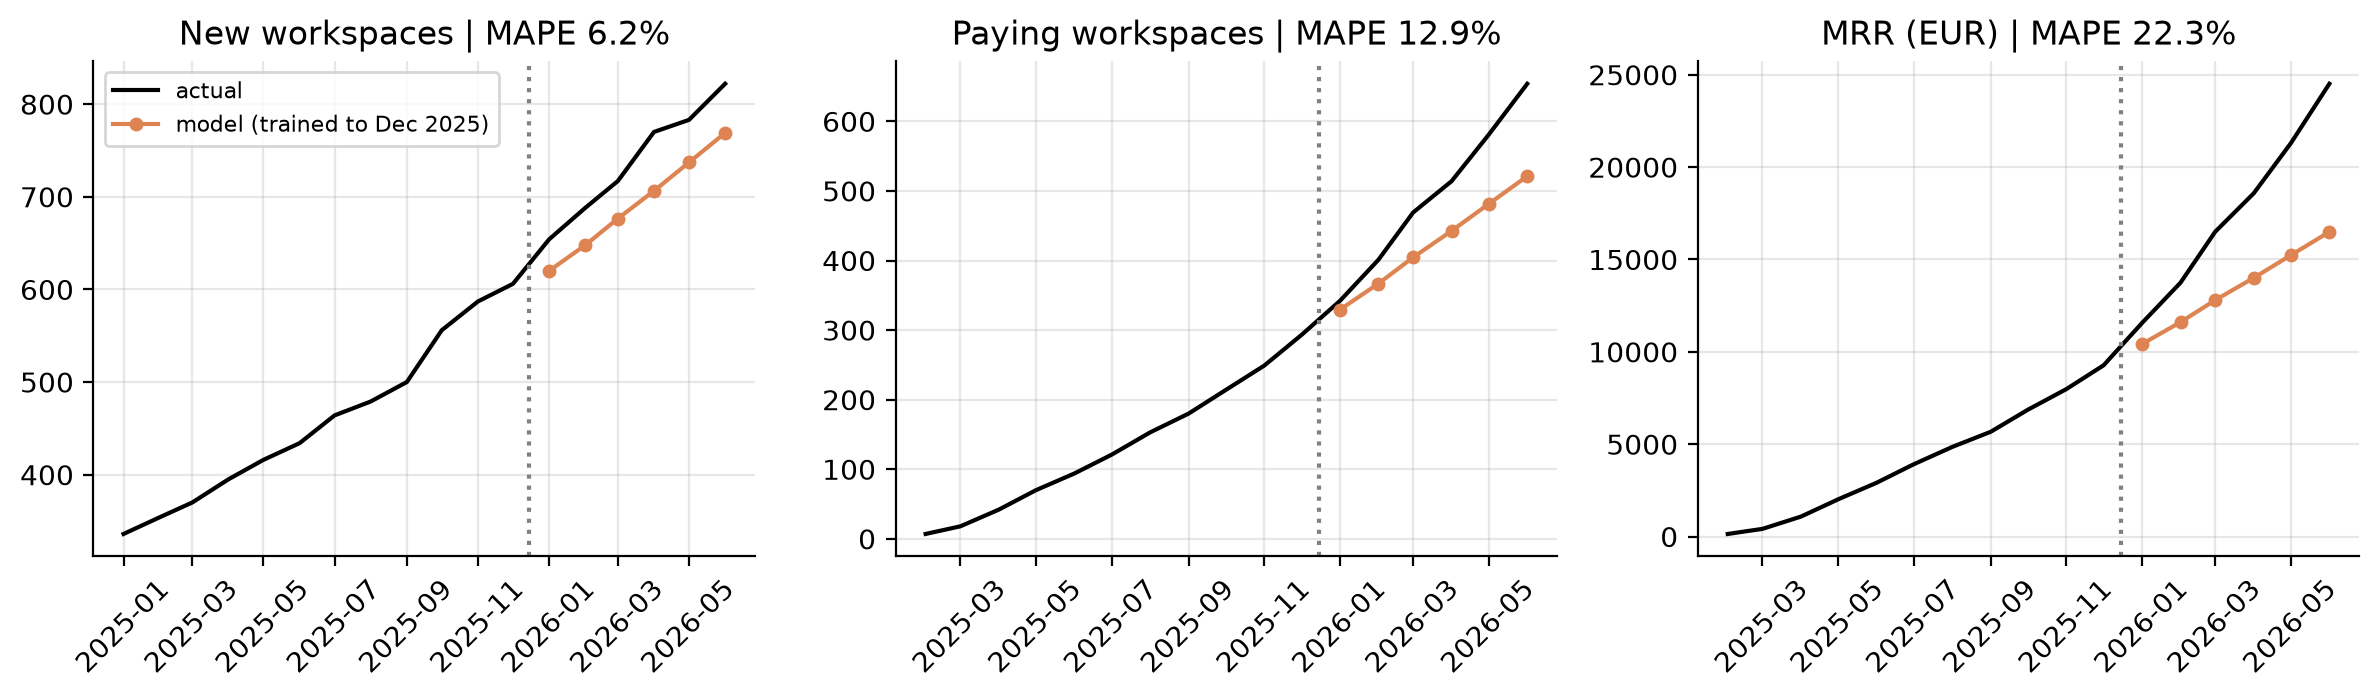
\includegraphics[width=0.96\textwidth]{fig14_backtest.png}
  \caption{Backtest: model calibrated on data up to 31 December 2025, simulated on Jan -- Jun 2026 with actual spend.}
  \label{fig:bt}
\end{figure}

\textbf{Backtest.} To test the model honestly, we calibrated it only on the data available on 31 December 2025, then let it run over the first half of 2026 with the spend actually incurred. It predicts acquisition well, with a mean absolute percentage error (MAPE) of \textbf{6.2\pc{}}, but it underestimates paying workspaces (\textbf{12.9\pc{}}) and MRR (\textbf{22.3\pc{}}), and the error widens month after month (Figure~\ref{fig:bt}). Breaking the error down shows where it comes from. In December 2025, the September onboarding change was still too recent to show up in mature 90-day cohorts, so the model was working with the old conversion rate. Giving it the post-change conversion brings the error on paying workspaces down to \textbf{4.0\pc{}}, and adding the ARPA observed in 2026 reduces the MRR error to \textbf{6.2\pc{}}. The model, in other words, is fragile exactly where the business changed, which is also where the board should look most carefully.

\begin{figure}[htbp]
  \centering
  \begin{subfigure}{0.49\textwidth}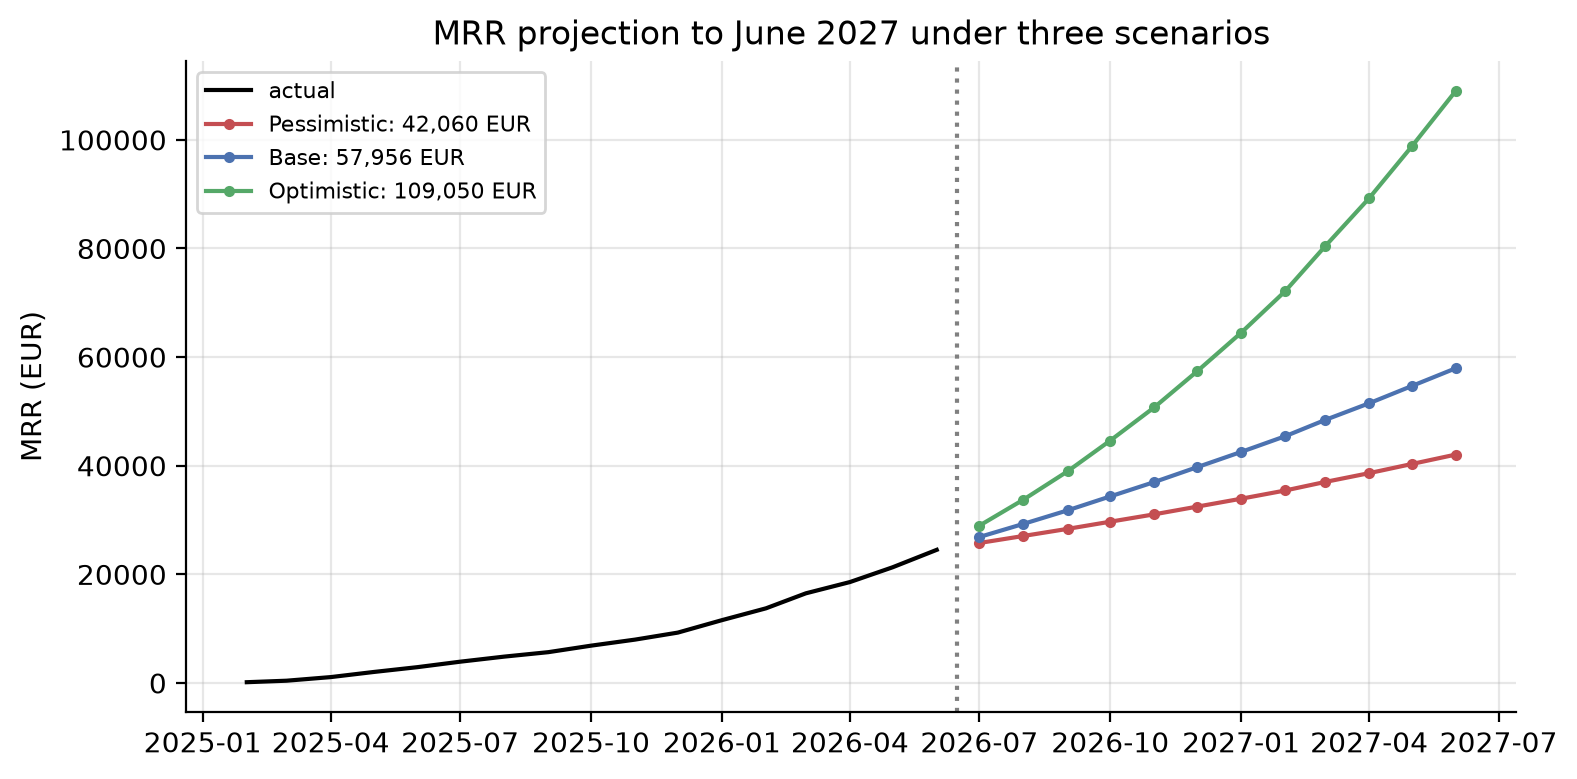
\includegraphics[width=\linewidth]{fig15_scenarios.png}\end{subfigure}\hfill
  \begin{subfigure}{0.48\textwidth}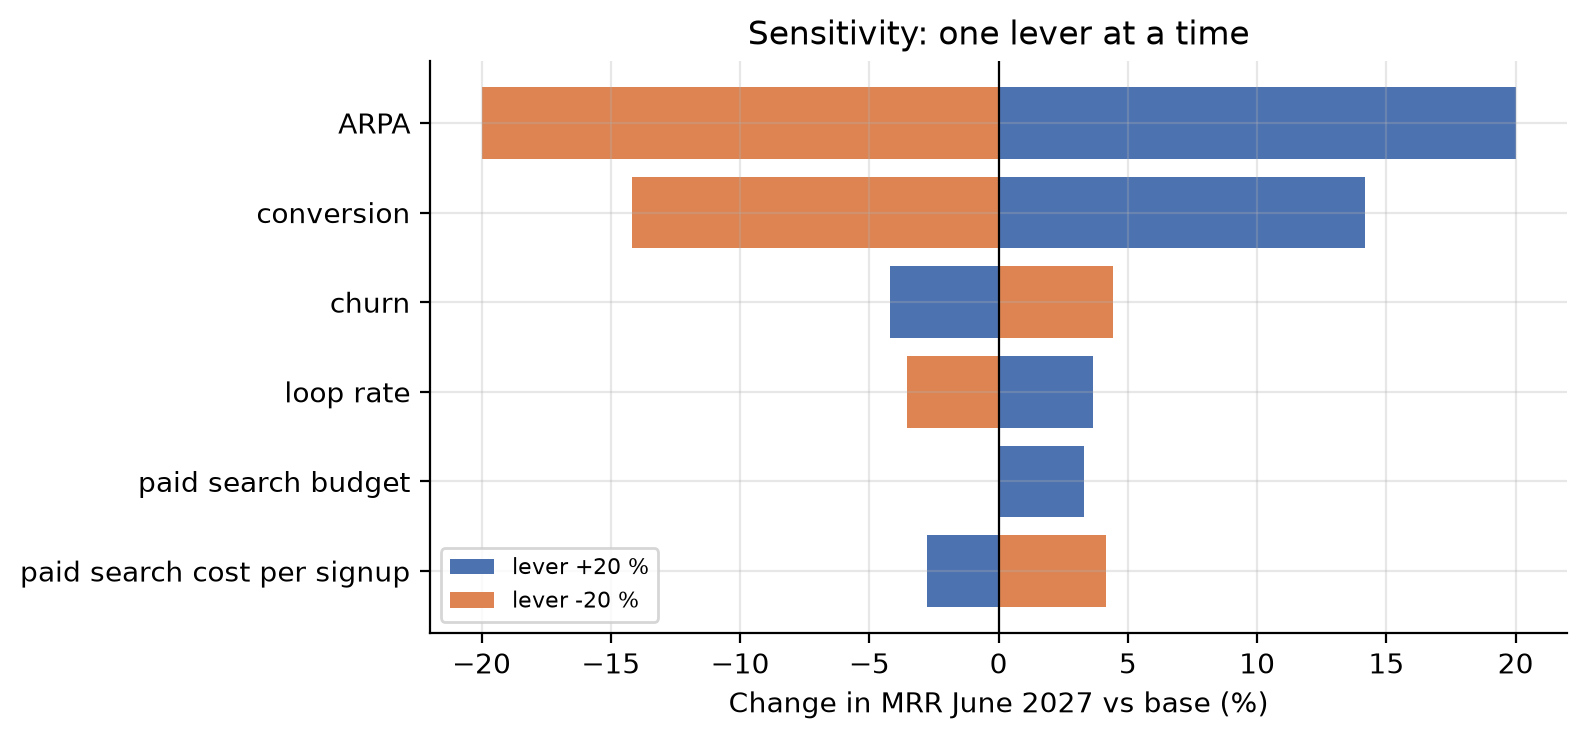
\includegraphics[width=\linewidth]{fig16_sensitivity.png}\end{subfigure}
  \caption{MRR projection to June 2027 under three scenarios (left) and sensitivity of June 2027 MRR to $\pm 20\pc{}$ lever shifts (right).}
  \label{fig:sc}
\end{figure}

\textbf{Scenarios (July 2026 -- June 2027).} The three scenarios keep the current spend trends and differ only in their levers, each of which takes a value already observed in the data rather than an assumed one (Figure~\ref{fig:sc}, left). The pessimistic scenario returns to the pre-change conversion (8.1\pc{}), applies the churn of small teams (4.4\pc{}) and the pre-change loop rate (1.7\pc{}). The base scenario keeps the post-change conversion (10.8\pc{}), the churn of the first half of 2026 (3.1\pc{}) and the current loop rate (2.0\pc{}). The optimistic scenario uses the conversion of activated workspaces after the change (14.4\pc{}), the churn of Business plans (2.1\pc{}), the best loop month on record (2.2\pc{}) and the ARPA trend of early 2026 (+2.9\pc{} a month). By June 2027, MRR reaches \textbf{42.1\,k\eur{}, 58.0\,k\eur{} and 109.1\,k\eur{}} respectively, that is an ARR of 0.50, 0.70 and 1.31\Meur. Yet the number of new workspaces hardly varies from one scenario to another (from 12.5\,k to 13.5\,k): the outcome is decided after the sign-up. The sensitivity analysis says the same thing (Figure~\ref{fig:sc}, right). Raising ARPA or conversion by 20\pc{} increases MRR by 20.0\pc{} and 14.2\pc{}, whereas the same increase in paid search budget adds only 3.3\pc{}.

% ==================================================================
\section{A/B test plan and recommendations}
\label{sec:ab}

The analysis leaves one question open: can paid search users be brought to form teams, as the other channels do? We propose to answer it with a controlled experiment. Our hypothesis is that a guided and optional ``Invite two teammates'' step, shown to paid search sign-ups before they create their first project, will raise their 30-day activation and, in turn, their 90-day conversion.
\begin{itemize}[nosep,topsep=2pt]
  \item \textbf{Design and metrics}: new \texttt{paid\_search} workspaces are split 50/50 at creation. The primary metric is 30-day activation (baseline 34.5\pc{}), the secondary metric is 90-day conversion (baseline 6.5\pc{}), and the guardrails are the churn of paying workspaces and the number of seats per workspace.
  \item \textbf{Sizing}: we use a two-sided test on two proportions, with $\alpha = 5\pc{}$ and a power of 80\pc{}. Paid search brings about 204 sign-ups a month, so detecting an 8-point lift in activation requires \textbf{577 workspaces per arm}, roughly 5.7 months of traffic plus 30 days of observation. Such an effect is plausible, since the September 2025 change already moved paid search activation by 11 points. A 5-point lift would take 14 months to detect, and a 2-point lift in conversion more than two years: activation is the only realistic primary metric, while conversion remains the commercial check that matters in the end.
  \item \textbf{Ethics}: the step must stay optional and transparent, with no forced sharing, no dark patterns and no automatic invitation of the user's contacts.
\end{itemize}

\begin{synthese}
\small
\begin{enumerate}[nosep,topsep=2pt,leftmargin=1.4em]
  \item \textbf{Adopt the team of three as North Star Metric}, and judge product and marketing initiatives by their effect on it.
  \item \textbf{Hold paid search spend at its current level} until the A/B test shows that its users can be activated and converted, and \textbf{direct any additional budget to content SEO}, the only paid channel close to 3\,:\,1 (2.86, 9.5-month payback, falling cost per sign-up).
  \item \textbf{Stop or renegotiate the partner programme} (LTV\,:\,CAC of 0.69 on revenue), for instance towards a fee paid per activated team.
  \item \textbf{Invest in activation and seat expansion}, which improve conversion, ARPA, retention and the guest loop at the same time.
\end{enumerate}
\end{synthese}

% ==================================================================
\newpage
\appendix
\section{Data cleaning log}
\label{sec:app-log}

\begin{table}[htbp]
\centering\footnotesize\renewcommand{\arraystretch}{1.15}
\begin{tabularx}{\linewidth}{@{}llXrl@{}}
\toprule
\# & Table & Cleaning rule / check applied & Rows & Action \\
\midrule
1  & workspaces & Internal test account (\texttt{W\_INTERNAL}, channel \texttt{internal}) & 1 & removed \\
2  & workspaces & Inconsistent \texttt{company\_size} labels (\texttt{1–10}, \texttt{11 to 50}, \texttt{11–50}) & 859 & harmonised \\
3  & workspaces & Missing \texttt{company\_size} value & 267 & set to \texttt{unknown} \\
4  & workspaces & \texttt{invite\_loop} workspace created before its \texttt{origin\_workspace\_id} & 66 & kept, excluded from loop timing \\
5  & users & Exact duplicate rows & 474 & removed \\
6  & users & Users belonging to the removed internal workspace (\texttt{W\_INTERNAL}) & 140 & removed \\
7  & users & \texttt{joined\_date} formatted as \texttt{DD/MM/YYYY} instead of ISO & 956 & converted to ISO \\
8  & users & \texttt{invited\_by\_user\_id} not found in \texttt{users} table & 1,591 & kept (membership valid) \\
9  & revenue & Exact duplicate billing rows & 22 & removed \\
10 & revenue & Negative \texttt{mrr\_eur} values (all equal to $-\text{seats} \times \text{list price}$, sign error) & 25 & replaced by $|\text{MRR}|$ \\
11 & revenue & Upgraded workspaces with no invoice (all upgraded in June 2026, billed from July) & 76 & kept (normal 1-month billing lag) \\
12 & all tables & Zero-violation checks: upgrade before creation or after 30/06/2026, plan without upgrade date, duplicate \texttt{user\_id} after dedup, user joined before workspace creation or after extraction, double monthly billing, $|\text{MRR}| \neq \text{seats} \times \text{price}$, revenue on free workspace, missing/negative spend & 0 & verified (0 rows affected) \\
\bottomrule
\end{tabularx}
\caption{Complete data cleaning log. Final clean dataset: 9,931 workspaces, 47,287 users, 4,402 invoices, and 54 marketing spend rows.}
\label{tab:log}
\end{table}

\end{document}
